% Options for packages loaded elsewhere
% Options for packages loaded elsewhere
\PassOptionsToPackage{unicode}{hyperref}
\PassOptionsToPackage{hyphens}{url}
\PassOptionsToPackage{dvipsnames,svgnames,x11names}{xcolor}
%
\documentclass[
  spanish,
  11pt,
  letterpaper,
  DIV=11,
  numbers=noendperiod]{scrartcl}
\usepackage{xcolor}
\usepackage[left=3cm,right=3cm,top=3cm,bottom=3cm]{geometry}
\usepackage{amsmath,amssymb}
\setcounter{secnumdepth}{-\maxdimen} % remove section numbering
\usepackage{iftex}
\ifPDFTeX
  \usepackage[T1]{fontenc}
  \usepackage[utf8]{inputenc}
  \usepackage{textcomp} % provide euro and other symbols
\else % if luatex or xetex
  \usepackage{unicode-math} % this also loads fontspec
  \defaultfontfeatures{Scale=MatchLowercase}
  \defaultfontfeatures[\rmfamily]{Ligatures=TeX,Scale=1}
\fi
\usepackage{lmodern}
\ifPDFTeX\else
  % xetex/luatex font selection
\fi
% Use upquote if available, for straight quotes in verbatim environments
\IfFileExists{upquote.sty}{\usepackage{upquote}}{}
\IfFileExists{microtype.sty}{% use microtype if available
  \usepackage[]{microtype}
  \UseMicrotypeSet[protrusion]{basicmath} % disable protrusion for tt fonts
}{}
\makeatletter
\@ifundefined{KOMAClassName}{% if non-KOMA class
  \IfFileExists{parskip.sty}{%
    \usepackage{parskip}
  }{% else
    \setlength{\parindent}{0pt}
    \setlength{\parskip}{6pt plus 2pt minus 1pt}}
}{% if KOMA class
  \KOMAoptions{parskip=half}}
\makeatother
% Make \paragraph and \subparagraph free-standing
\makeatletter
\ifx\paragraph\undefined\else
  \let\oldparagraph\paragraph
  \renewcommand{\paragraph}{
    \@ifstar
      \xxxParagraphStar
      \xxxParagraphNoStar
  }
  \newcommand{\xxxParagraphStar}[1]{\oldparagraph*{#1}\mbox{}}
  \newcommand{\xxxParagraphNoStar}[1]{\oldparagraph{#1}\mbox{}}
\fi
\ifx\subparagraph\undefined\else
  \let\oldsubparagraph\subparagraph
  \renewcommand{\subparagraph}{
    \@ifstar
      \xxxSubParagraphStar
      \xxxSubParagraphNoStar
  }
  \newcommand{\xxxSubParagraphStar}[1]{\oldsubparagraph*{#1}\mbox{}}
  \newcommand{\xxxSubParagraphNoStar}[1]{\oldsubparagraph{#1}\mbox{}}
\fi
\makeatother


\usepackage{longtable,booktabs,array}
\newcounter{none} % for unnumbered tables
\usepackage{calc} % for calculating minipage widths
% Correct order of tables after \paragraph or \subparagraph
\usepackage{etoolbox}
\makeatletter
\patchcmd\longtable{\par}{\if@noskipsec\mbox{}\fi\par}{}{}
\makeatother
% Allow footnotes in longtable head/foot
\IfFileExists{footnotehyper.sty}{\usepackage{footnotehyper}}{\usepackage{footnote}}
\makesavenoteenv{longtable}
\usepackage{graphicx}
\makeatletter
\newsavebox\pandoc@box
\newcommand*\pandocbounded[1]{% scales image to fit in text height/width
  \sbox\pandoc@box{#1}%
  \Gscale@div\@tempa{\textheight}{\dimexpr\ht\pandoc@box+\dp\pandoc@box\relax}%
  \Gscale@div\@tempb{\linewidth}{\wd\pandoc@box}%
  \ifdim\@tempb\p@<\@tempa\p@\let\@tempa\@tempb\fi% select the smaller of both
  \ifdim\@tempa\p@<\p@\scalebox{\@tempa}{\usebox\pandoc@box}%
  \else\usebox{\pandoc@box}%
  \fi%
}
% Set default figure placement to htbp
\def\fps@figure{htbp}
\makeatother



\ifLuaTeX
\usepackage[bidi=basic,shorthands=off]{babel}
\else
\usepackage[bidi=default,shorthands=off]{babel}
\fi
\ifLuaTeX
  \usepackage{selnolig} % disable illegal ligatures
\fi


\setlength{\emergencystretch}{3em} % prevent overfull lines

\providecommand{\tightlist}{%
  \setlength{\itemsep}{0pt}\setlength{\parskip}{0pt}}



 


\usepackage{booktabs}
\usepackage{longtable}
\usepackage{array}
\usepackage{multirow}
\usepackage{wrapfig}
\usepackage{float}
\usepackage{colortbl}
\usepackage{pdflscape}
\usepackage{tabularx}
\usepackage{xltabular}
\usepackage{threeparttable}
\usepackage{threeparttablex}
\usepackage[normalem]{ulem}
\usepackage{makecell}
\usepackage{xcolor}
\KOMAoption{captions}{tableheading}
\usepackage{caption}
\captionsetup[table]{position=bottom,labelformat=default,labelsep=colon,name=Tabla}
\captionsetup[figure]{labelformat=default,labelsep=colon,name=Figura}
\usepackage{float}
\floatplacement{figure}{H}
\makeatletter
\@ifpackageloaded{caption}{}{\usepackage{caption}}
\AtBeginDocument{%
\ifdefined\contentsname
  \renewcommand*\contentsname{Tabla de contenidos}
\else
  \newcommand\contentsname{Tabla de contenidos}
\fi
\ifdefined\listfigurename
  \renewcommand*\listfigurename{Listado de Figuras}
\else
  \newcommand\listfigurename{Listado de Figuras}
\fi
\ifdefined\listtablename
  \renewcommand*\listtablename{Listado de Tablas}
\else
  \newcommand\listtablename{Listado de Tablas}
\fi
\ifdefined\figurename
  \renewcommand*\figurename{Figura}
\else
  \newcommand\figurename{Figura}
\fi
\ifdefined\tablename
  \renewcommand*\tablename{Tabla}
\else
  \newcommand\tablename{Tabla}
\fi
}
\@ifpackageloaded{float}{}{\usepackage{float}}
\floatstyle{ruled}
\@ifundefined{c@chapter}{\newfloat{codelisting}{h}{lop}}{\newfloat{codelisting}{h}{lop}[chapter]}
\floatname{codelisting}{Listado}
\newcommand*\listoflistings{\listof{codelisting}{Listado de Listados}}
\makeatother
\makeatletter
\makeatother
\makeatletter
\@ifpackageloaded{caption}{}{\usepackage{caption}}
\@ifpackageloaded{subcaption}{}{\usepackage{subcaption}}
\makeatother
\usepackage{bookmark}
\IfFileExists{xurl.sty}{\usepackage{xurl}}{} % add URL line breaks if available
\urlstyle{same}
\hypersetup{
  pdflang={es-ES},
  colorlinks=true,
  linkcolor={blue},
  filecolor={Maroon},
  citecolor={Blue},
  urlcolor={Blue},
  pdfcreator={LaTeX via pandoc}}


\author{}
\date{}
\begin{document}


\begin{titlepage}
    \centering
    % Logo
    
\includegraphics[width=0.7\textwidth]{logo_facultad.png}\par
    % Espacio entre logo y título principal
    \vspace{3cm}
    % Título principal
    {\scshape\Huge Trabajo Práctico de Modelos Lineales Generalizados \par}
    \vfill
    % Carrera y Alumnos
    {\Large Integrantes: \\[0.15cm]
     Cañizares María Inés \\[0.15cm]
     Zame, Lisbeth \par}
    \vspace{1cm}
    {\Large Licenciatura en Estadística \par}
    % Fecha abajo del todo
    \vspace{0.15cm}
    {\large Año 2026 \par}
\end{titlepage}

\section{Introducción}\label{introducciuxf3n}

El hundimiento del RMS Titanic, ocurrido en 1912 durante su viaje
inaugural, es una de las tragedias marítimas más recordadas de la
historia. Considerado el mayor transatlántico de su época y casi
insumergible, su naufragio causó la muerte de más de 1.500 de las
aproximadamente 2.200 personas a bordo y dejó en evidencia graves
falencias de seguridad, como la escasez de botes salvavidas. El suceso
provocó una conmoción mundial e impulsó cambios en la normativa
internacional. Los datos de sus pasajeros permiten, además, estudiar si
la supervivencia estuvo asociada a características individuales como el
sexo, la edad, la tarifa abonada o el puerto de embarque, y contrastar
con evidencia empírica la norma de ``mujeres y niños primero''.

En este trabajo se busca identificar los factores con mayor influencia
en la probabilidad de supervivencia de los pasajeros, mediante un Modelo
Lineal Generalizado sobre la base de datos del Titanic construida a
partir de registros históricos reales.

\section{Material y métodos}\label{material-y-muxe9todos}

En este contexto, el presente trabajo tiene como objetivo modelar la
probabilidad de supervivencia de los pasajeros del Titanic en función de
sus características individuales, mediante un Modelo Lineal Generalizado
con función de enlace logit. Este enfoque, permite estimar el efecto de
cada variable en términos de razones de odds y evaluar posibles
interacciones entre ellas.

La base de datos utilizada contiene información de 891 pasajeros. Dado
que presentaba datos faltantes, se optó por eliminar las observaciones
incompletas, por lo que el análisis se realizó sobre 712 observaciones.
Para evaluar la capacidad predictiva del modelo, esta base se dividió en
dos subconjuntos: uno de entrenamiento, con 571 observaciones, utilizado
para ajustar el modelo, y uno de prueba, con las 141 restantes,
reservado para evaluar su desempeño predictivo sobre datos no utilizados
en el ajuste.

La variable respuesta es Survived, que indica si el pasajero sobrevivió
al naufragio: toma el valor 1 si sobrevivió (SÍ) y 0 si no sobrevivió
(NO). Al tratarse de una variable binaria, se asume que cada observación
sigue una distribución Bernoulli.

El análisis comenzó con un estudio descriptivo de las variables, para
explorar su distribución y su relación con la supervivencia. Luego se
seleccionaron las variables del modelo sobre el conjunto de
entrenamiento y se ajustó el modelo final con enlace logit. Se evaluó su
ajuste y su capacidad predictiva sobre el conjunto de prueba. Por
último, se compararon distintas funciones de enlace (logit, probit y
cloglog), con el fin de identificar qué factores estuvieron más
fuertemente asociados a la supervivencia.

Las variables explicativas incluidas en el análisis se describen a
continuación:

\begin{itemize}
  \item \textbf{Edad}: medida en años. Es una variable cuantitativa continua.

 \item \textbf{Tarifa}: precio del pasaje abonado por el pasajero, medida en libras esterlinas (£). Es una variable cuantitativa continua.
 
 \item \textbf{Embarcación}: puerto en el que el pasajero abordó el Titanic, categorizada en tres niveles:
  \begin{itemize}
    \item ``C'': Cherburgo (Francia)
    \item ``Q'': Queenstown (Irlanda, actual Cobh)
    \item ``S'': Southampton (Inglaterra)
  \end{itemize}

  \item \textbf{Sexo}: sexo del pasajero. Fue categorizada en dos niveles:
  \begin{itemize}
    \item “Male”: Masculino
    \item “female”: Femenino
  \end{itemize}
\end{itemize}

\section{Análisis Descriptivo}\label{anuxe1lisis-descriptivo}

A continuación se presenta una visión general de las características
clave de la población estudiada.

\begin{table}[!h]
\centering
\caption{\label{tab:unnamed-chunk-3}Frecuencias absolutas y relativas de supervivencia}
\centering
\begin{tabular}[t]{ccc}
\toprule
Sobrevivió & Frecuencia & Porcentaje (\%)\\
\midrule
No & 424 & 59.55\\
Sí & 288 & 40.45\\
Total & 712 & 100.00\\
\bottomrule
\end{tabular}
\end{table}

\section{\texorpdfstring{\texttt{\{r,\ eval=FALSE\}\ \#\ \#\ resumen\ general\ de\ variables\ \#\ skim(datos)\ \#}}{\{r, eval=FALSE\} \# \# resumen general de variables \# skim(datos) \#}}\label{r-evalfalse-resumen-general-de-variables-skimdatos}

\begin{table}[!h]
\centering
\caption{\label{tab:unnamed-chunk-4}Frecuencias absolutas y relativas de sexo}
\centering
\begin{tabular}[t]{ccc}
\toprule
Sexo & Frecuencia & Porcentaje (\%)\\
\midrule
Femenino & 259 & 36.38\\
Masculino & 453 & 63.62\\
Total & 712 & 100\\
\bottomrule
\end{tabular}
\end{table}

\begin{table}[!h]
\centering
\caption{\label{tab:unnamed-chunk-5}Frecuencias absolutas y relativas de Embarcación}
\centering
\begin{tabular}[t]{ccc}
\toprule
Embarcación & Frecuencia & Porcentaje (\%)\\
\midrule
C & 130 & 18.26\\
Q & 28 & 3.93\\
S & 554 & 77.81\\
Total & 712 & 100\\
\bottomrule
\end{tabular}
\end{table}

\begin{table}[!h]
\centering
\caption{\label{tab:unnamed-chunk-6}Estadísticas descriptivas de la variable edad}
\centering
\begin{tabular}[t]{cccccc}
\toprule
Variable & Media & Mediana & DE & Mínimo & Máximo\\
\midrule
edad & 29.64 & 28 & 14.49 & 0.42 & 80\\
\bottomrule
\end{tabular}
\end{table}

\begin{table}[!h]
\centering
\caption{\label{tab:unnamed-chunk-7}Estadísticas descriptivas de la variable edad}
\centering
\begin{tabular}[t]{cccccc}
\toprule
Variable & Media & Mediana & DE & Mínimo & Máximo\\
\midrule
tarifa & 34.57 & 15.64585 & 52.94 & 0 & 512.3292\\
\bottomrule
\end{tabular}
\end{table}

\section{FALTAN CONCLUSIONES DE TABLAS DESPUES DE
REPRODUCIR}\label{faltan-conclusiones-de-tablas-despues-de-reproducir}

\begin{figure}

\centering{

\pandocbounded{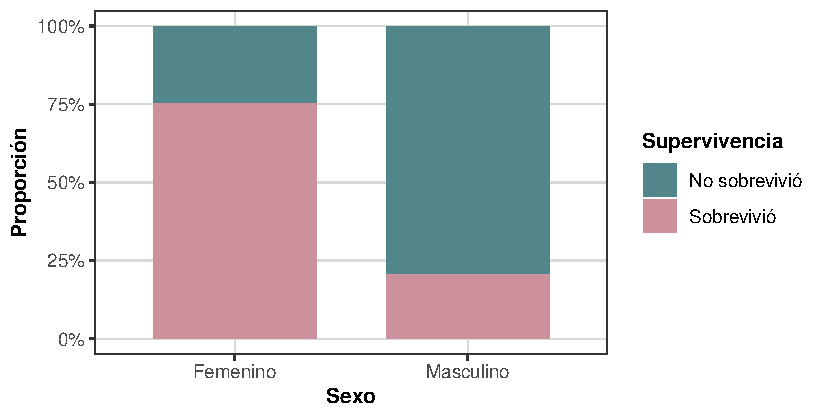
\includegraphics[keepaspectratio]{TpMLG_files/figure-pdf/fig-1-1.pdf}}

}

\caption{\label{fig-1}Proporción de pasajeros sobrevivientes según sexo}

\end{figure}%

Se observa que la proporción de pasajeros que sobrevivieron es más alta
para aquellos con sexo femenino en comparacón a los pasajeros
masculinos.

\begin{figure}

\centering{

\pandocbounded{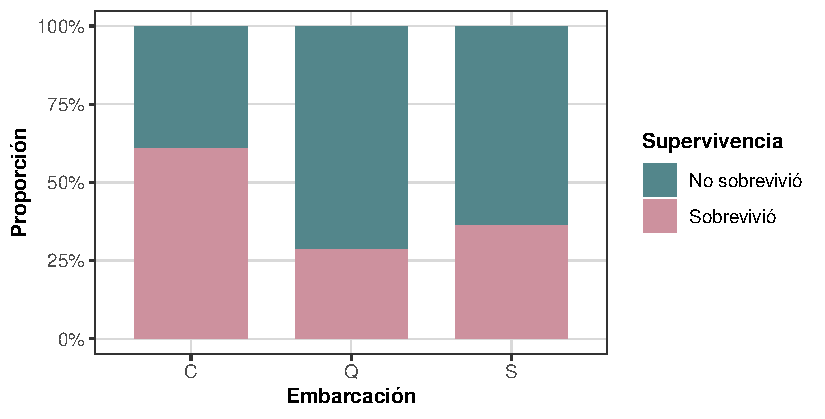
\includegraphics[keepaspectratio]{TpMLG_files/figure-pdf/fig-2-1.pdf}}

}

\caption{\label{fig-2}Proporción de pasajeros sobrevivientes según lugar
de embarcación}

\end{figure}%

Se observa una mayor proporción de sobrevivientes entre los pasajeros
que embarcaron en C (aprox. 60\%) en comparación con Q y S (aprox. 28\%
y 36\%), lo que sugiere una posible asociación entre el puerto de
embarque y la supervivencia.

Graficos de la variable edad

\begin{figure}[H]

{\centering \pandocbounded{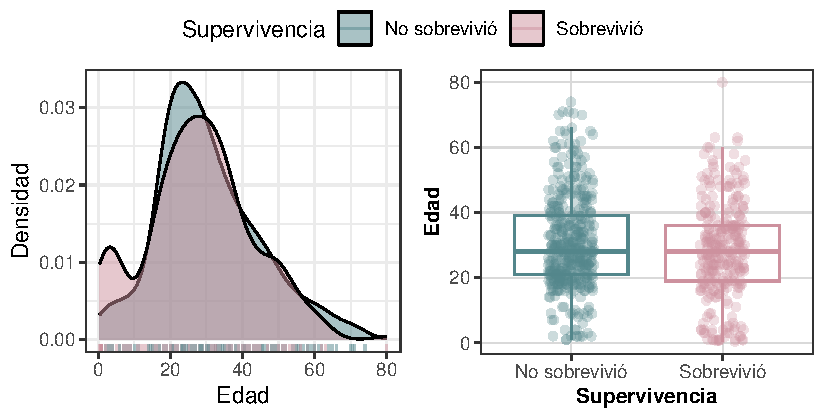
\includegraphics[keepaspectratio]{TpMLG_files/figure-pdf/unnamed-chunk-8-1.pdf}}

}

\caption{Distribución de la edad según supervivencia}

\end{figure}%

La distribución de la edad es similar entre sobrevivientes y no
sobrevivientes, con medianas casi idénticas (aprox. 28 años), por lo que
la edad parece no estar fuertemente asociada a la supervivencia. Se
observa, sin embargo, una mayor proporción de sobrevivientes entre los
niños pequeños, y una leve mayor presencia de no sobrevivientes en
edades avanzadas.

GRaficos de la variable Tarifa

\begin{figure}[H]

{\centering \pandocbounded{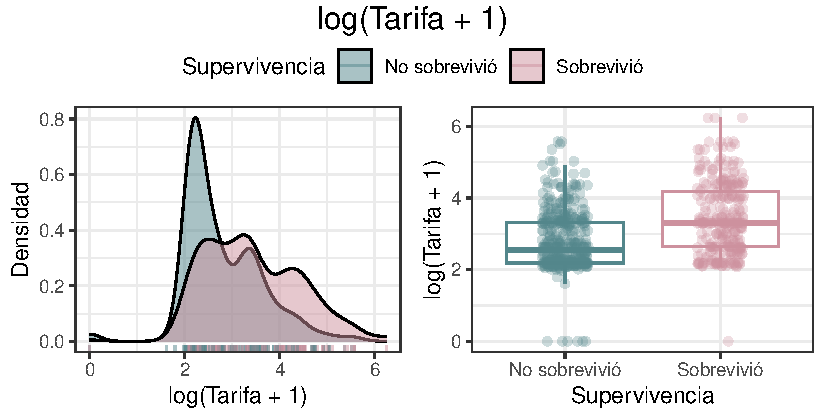
\includegraphics[keepaspectratio]{TpMLG_files/figure-pdf/unnamed-chunk-9-1.pdf}}

}

\caption{Distribución de la log(Tarifa) según supervivencia}

\end{figure}%

La tarifa pagada parece estar asociada a la supervivencia: los pasajeros
que sobrevivieron presentan en general tarifas más altas (mediana de
log(Tarifa + 1) mayor) que quienes no sobrevivieron, que se concentran
en tarifas bajas. Esto sugiere que la tarifa podría ser un predictor
relevante de la supervivencia.

\section{Modelado estadístico}\label{modelado-estaduxedstico}

El trabajo se realizará bajo el enfoque de modelos lineales
generalizados, utilizando lo desarrollado por Nelder y Wedderburn.

\subsection{Selección del modelo}\label{selecciuxf3n-del-modelo}

Para modelar la probabilidad de supervivencia de los pasajeros del
Titanic, en función de las variables explicativas sexo, edad, tarifa del
pasaje y puerto de embarque, se propuso emplear un modelo con función de
enlace logit.

En primer lugar, se seleccionaron las variables explicativas
consideradas relevantes para explicar la supervivencia de los pasajeros
y se ajustó un modelo que incluyó sus efectos principales. A
continuación, se evaluó la incorporación de interacciones de segundo
orden entre dichas variables, utilizando los métodos de selección hacia
adelante (forward) y hacia atrás (backward), con el criterio de
información de Akaike (AIC) y la deviance de cada modelo. Ambos
procedimientos condujeron al mismo modelo final, que incorpora las
interacciones entre sexo y edad, y entre edad y tarifa del pasaje.

\section{Probamos linealidad de la predictoras
continuas}\label{probamos-linealidad-de-la-predictoras-continuas}

Con el objetivo de evaluar si la relación entre la edad y el logit de la
probabilidad de supervivencia podía considerarse lineal, se compararon
dos modelos alternativos.

En primer lugar, se construyó un modelo que incorpora la variable edad
como ordinal, dividiendo su rango en cinco categorías según los
cuantiles 0.2, 0.4, 0.6 y 0.8. Posteriormente, se ajustó un segundo
modelo en el que la edad se representó mediante variables indicadoras
(dummies), permitiendo una relación no necesariamente lineal con la
respuesta.

El modelo ordinal se puede expresar como:

\[
\quad \text{logit}(\pi_i) =
\beta_0 + \beta_1\,\text{Sexo}_i +
\beta_2\,\text{logTarifa}_i +
\beta_3\,\text{EmbarcacionQ}_i +
\beta_4\,\text{EmbarcacionS}_i +
\beta_5\,\text{Edad}_i + 
\beta_6\, (\text{Sexo}_i \times \text{Edad}_i) +
\beta_7\, (\text{logTarifa}_i \times \text{Edad}_i)
\]

Mientras que el modelo con variables indicadoras se define como:

\[
\begin{aligned}
\text{logit}(\pi_i) = & \, \beta_0 + \beta_1\,\text{Sexo}_i + \beta_2\,\text{logTarifa}_i + \beta_3\,\text{EmbarcacionQ}_i + \beta_4\,\text{EmbarcacionS}_i \\
& + \beta_5\,\text{Edad2}_i + \beta_6\,\text{Edad3}_i + \beta_7\,\text{Edad4}_i + \beta_8\,\text{Edad5}_i \\
& + \beta_9\,(\text{Sexo}_i \times \text{Edad2}_i) + \beta_{10}\,(\text{Sexo}_i \times \text{Edad3}_i) + \beta_{11}\,(\text{Sexo}_i \times \text{Edad4}_i) + \beta_{12}\,(\text{Sexo}_i \times \text{Edad5}_i) \\
& + \beta_{13}\,(\text{logTarifa}_i \times \text{Edad2}_i) + \beta_{14}\,(\text{logTarifa}_i \times \text{Edad3}_i) + \beta_{15}\,(\text{logTarifa}_i \times \text{Edad4}_i) + \beta_{16}\,(\text{logTarifa}_i \times \text{Edad5}_i)
\end{aligned}
\]

Finalmente, se evaluó si la incorporación de esta última variable
aportaba una mejora significativa al modelo original mediante una prueba
de razón de verosimilitudes.

Los resultados no proporcionaron evidencia suficiente para justificar la
incorporación de la edad categorizada (\(p-value = 0.19\)). Por lo
tanto, se decidió mantener la edad como variable continua en el modelo
final.

Adicionalmente, dado que se cuenta con otra variable continua clave como
el logaritmo de la tarifa (logTarifa), se procedió a evaluar de forma
análoga si su relación con el logit de la probabilidad de supervivencia
podía considerarse lineal mediante la comparación de modelos
alternativos.

En primer lugar, se construyó un modelo que incorpora la variable
logTarifa como ordinal, dividiendo su rango en cinco categorías según
los cuantiles 0.2, 0.4, 0.6 y 0.8. Posteriormente, se ajustó un segundo
modelo en el que dicha variable se representó mediante variables
indicadoras (dummies), permitiendo capturar una relación no
necesariamente lineal con la respuesta.

El modelo ordinal se puede expresar como:

\[
\quad \text{logit}(\pi_i) =
\beta_0 + \beta_1\,\text{Sexo}_i +
\beta_2\,\text{logTarifa}_i +
\beta_3\,\text{EmbarcacionQ}_i +
\beta_4\,\text{EmbarcacionS}_i +
\beta_5\,\text{Edad}_i + 
\beta_6\, (\text{Sexo}_i \times \text{Edad}_i) +
\beta_7\, (\text{logTarifa}_i \times \text{Edad}_i)
\] Mientras que el modelo con variables indicadoras se define como:

\$\$ \quad \text{logit}(\pi\_i) = \beta\_0 + \beta\_1,\text{Sexo}\_i +
\beta\_2,\text{Edad}\_i + \beta\_3,\text{EmbarcacionQ}\_i +
\beta\_4,\text{EmbarcacionS}\_i + \beta\_5,\text{logTarifa2}\_i +
\beta\_6,\text{logTarifa3}\_i + \beta\_7,\text{logTarifa4}\_i +
\beta\_8,\text{logTarifa5}\_i + \beta\_9, (\text{Sexo}\_i
\times \text{Edad}\_i) + \beta\_10,(\text{logTarifa2}\_i
\times \text{Edad}\_i) + \beta\_11,(\text{logTarifa3}\_i
\times \text{Edad}\_i) + \beta\_12, (\text{logTarifa4}\_i
\times \text{Edad}\_i) + \beta\_13, (\text{logTarifa5}\_i
\times \text{Edad}\_i)

\$\$ Los resultados no proporcionaron evidencia suficiente para
justificar la incorporación de la tarifa categorizada de forma no lineal
(\(p-value = 0.56\)). Por lo tanto, se decidió mantener logTarifa como
variable continua en el modelo final.

Por lo tanto, el modelo seleccionado se expresa como:

\[
\text{logit}(\pi_i) = \ln\left(\frac{\pi_i}{1 - \pi_i}\right) =
\beta_0 + \beta_1\,\text{Sexo}_i +
\beta_2\,\text{logTarifa}_i +
\beta_3\,\text{EmbarcacionQ}_i +
\beta_4\,\text{EmbarcacionS}_i +
\beta_5\,\text{Edad}_i + 
\beta_6\, (\text{Sexo}_i \times \text{Edad}_i) +
\beta_7\, (\text{logTarifa}_i \times \text{Edad}_i), \quad i=\overline{1,571}
\]

\begin{verbatim}

Call:
glm(formula = Survived ~ Sex + logFare + Embarked + Age + Sex:Age + 
    logFare:Age, family = binomial("logit"), data = train)

Coefficients:
               Estimate Std. Error z value Pr(>|z|)   
(Intercept)   -0.791618   1.035182  -0.765  0.44444   
Sexfemale      0.932122   0.485909   1.918  0.05507 . 
logFare        0.123888   0.298546   0.415  0.67816   
EmbarkedC      0.617034   0.286326   2.155  0.03116 * 
EmbarkedQ     -0.500167   0.598807  -0.835  0.40356   
Age           -0.094543   0.036600  -2.583  0.00979 **
Sexfemale:Age  0.050158   0.016786   2.988  0.00281 **
logFare:Age    0.018863   0.009998   1.887  0.05922 . 
---
Signif. codes:  0 '***' 0.001 '**' 0.01 '*' 0.05 '.' 0.1 ' ' 1

(Dispersion parameter for binomial family taken to be 1)

    Null deviance: 770.64  on 570  degrees of freedom
Residual deviance: 541.82  on 563  degrees of freedom
AIC: 557.82

Number of Fisher Scoring iterations: 5
\end{verbatim}

\noindent donde:

\begin{itemize}
  \item $\text{Sexo}_i = 
  \begin{cases}
    1 & \text{si } \text{Masculino} \\
    0 & \text{si } \text{Femenino} 
  \end{cases}$
  
  \item $\text{EmbarcaciónQ}_i = 
  \begin{cases}
    1 & \text{si } \text{Embarcación = Q}  \\
    0 & \text{si } \text{en otro caso} 
  \end{cases}$  

  \item $\text{EmbarcaciónS}_i = 
  \begin{cases}
    1 & \text{si } \text{Embarcación = S}  \\
    0 & \text{si } \text{en otro caso} 
  \end{cases}$
\end{itemize}

\subsection{Bondad del ajuste y estimación del
modelo}\label{bondad-del-ajuste-y-estimaciuxf3n-del-modelo}

\begin{verbatim}
Analysis of Deviance Table

Model 1: Survived ~ Sex + logFare + Embarked + Age + Sex:Age + logFare:Age
Model 2: Survived ~ Sex + logFare + Embarked + Age + eta2 + Sex:Age + 
    logFare:Age
  Resid. Df Resid. Dev Df Deviance Pr(>Chi)
1       563     541.82                     
2       562     539.36  1   2.4603   0.1168
\end{verbatim}

Se evalúa la adecuación de la función de enlace logit utilizada en el
modelo aplicando el test de especificación de la función de enlace, que
consiste en incorporar al modelo un término adicional cuadrático del
predictor lineal estimado:

\[
\begin{aligned}
M1)\quad \text{logit}(\pi_i) &= \beta_0 + \beta_1\,\text{Sexo}_i +
\beta_2\,\text{logTarifa}_i +
\beta_3\,\text{EmbarcacionQ}_i +
\beta_4\,\text{EmbarcacionS}_i +
\beta_5\,\text{Edad}_i + 
\beta_6\, (\text{Sexo}_i \times \text{Edad}_i) +
\beta_7\, (\text{logTarifa}_i \times \text{Edad}_i), \quad i=\overline{1,571}\\
M2)\quad \text{logit}(\pi_i) &= \beta_0 + \beta_1\,\text{Sexo}_i +
\beta_2\,\text{logTarifa}_i +
\beta_3\,\text{EmbarcacionQ}_i +
\beta_4\,\text{EmbarcacionS}_i +
\beta_5\,\text{Edad}_i + 
\beta_6\, (\text{Sexo}_i \times \text{Edad}_i) +
\beta_7\, (\text{logTarifa}_i \times \text{Edad}_i) + \hat{\eta}_i^2 \quad i=\overline{1,571}
\end{aligned}
\] El procedimiento implica ajustar un modelo extendido que incluye esta
nueva variable y comparar su ajuste con el modelo original mediante una
prueba de razón de verosimilitud. En este análisis, la comparación entre
ambos modelos no mostró evidencia suficiente para rechazar la adecuación
del enlace logit, por lo que se considera apropiado mantenerlo en el
modelo final (\(p-value = 0.12\)).

\begin{verbatim}

   The Hosmer-Lemeshow goodness-of-fit test

 Group Size Observed  Expected
     1   57        5  3.150576
     2   57        9  6.476041
     3   57        5  8.592194
     4   57        8 10.209854
     5   57       13 13.473276
     6   57       25 20.596549
     7   58       32 32.895530
     8   57       35 38.546529
     9   57       45 44.550668
    10   57       54 52.508783

         Statistic =  7.72829 
degrees of freedom =  8 
           p-value =  0.46045 
\end{verbatim}

Además, para evaluar la bondad de ajuste del modelo, se aplicó la prueba
de Hosmer y Lemeshow. Esta prueba compara las frecuencias observadas y
esperadas del evento de interés en grupos formados a partir de los
valores predichos por el modelo y dado el tamaño muestral disponible, se
optó por dividir las observaciones en 10 grupos de igual tamaño según
los valores de probabilidad predicha. Finalmente, se concluye que el
modelo presenta un ajuste adecuado a los datos (\(p-value = 0.46\)).

Considerando los resultados del estudio del modelo a través de los
diferentes tests de hipótesis, el ajuste realizado es el siguiente:

\[
\text{logit}(\hat{\pi_i}) = \ln\left(\frac{\hat{\pi_i}}{1 - \hat{\pi_i}}\right) = 0.76 - 0.93\,\text{Sexo}_i +
0.12\,\text{logTarifa}_i -
1.12\,\text{EmbarcacionQ}_i -
0.62\,\text{EmbarcacionS}_i -
0.045\,\text{Edad}_i - 
0.05\, (\text{Sexo}_i \times \text{Edad}_i) +
0.019\, (\text{logTarifa}_i \times \text{Edad}_i), \quad i=\overline{1,571}
\]

\begin{verbatim}
             df      AIC
modelo_final  8 557.8219
m_probit      8 557.9927
m_cloglog     8 554.4901
\end{verbatim}

\begin{center}
\pandocbounded{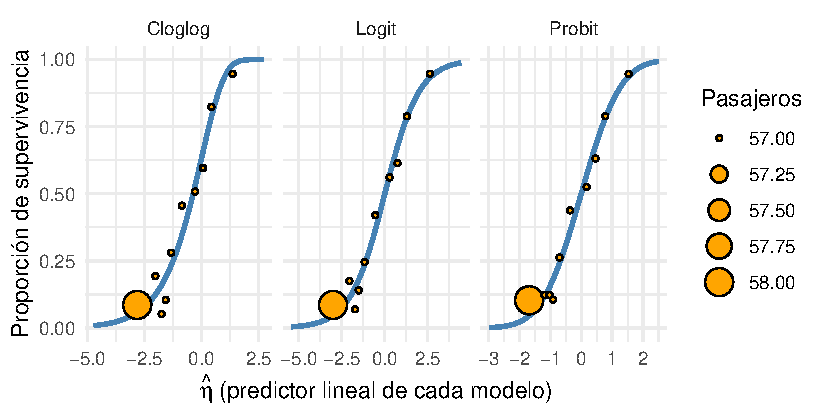
\includegraphics[keepaspectratio]{TpMLG_files/figure-pdf/unnamed-chunk-16-1.pdf}}
\end{center}

\subsection{Análisis de residuos}\label{anuxe1lisis-de-residuos}

El análisis de residuos permite evaluar la adecuación del modelo
ajustado, tanto en lo que respecta a la componente sistemática como a la
aleatoria.

Con el objetivo de analizar la estructura del modelo, se construyó el
gráfico de los residuos cuantil frente a las probabilidades estimadas
bajo el enlace logit.

\begin{figure}[H]

{\centering \pandocbounded{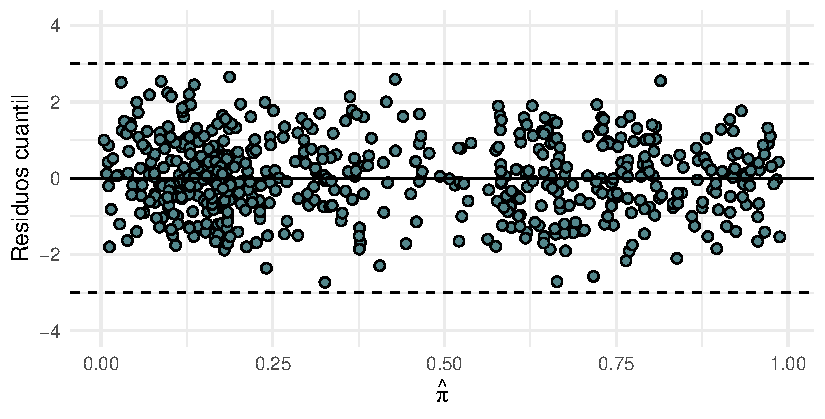
\includegraphics[keepaspectratio]{TpMLG_files/figure-pdf/unnamed-chunk-17-1.pdf}}

}

\caption{Gráfico de residuos cuantil vs.~las probabilidades estimadas}

\end{figure}%

En este gráfico se observa que los residuos se distribuyen
aproximadamente alrededor de cero, sin evidenciar un patrón sistemático
definido. Si bien se observa una mayor concentración de observaciones en
el rango de probabilidades estimadas más bajas, no se identifican
tendencias claras que indiquen problemas importantes de ajuste. Esto
sugiere que la función de enlace logit es adecuada y que el modelo logra
capturar correctamente la relación entre las variables explicativas y la
probabilidad de sobrevivir.

Además, para verificar la adecuación de la distribución supuesta de los
errores, se empleó un gráfico QQ de los residuos cuantil.

\begin{figure}[H]

{\centering \pandocbounded{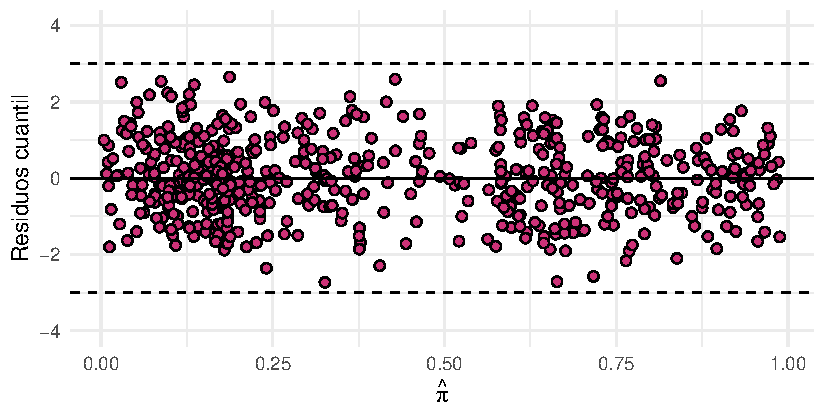
\includegraphics[keepaspectratio]{TpMLG_files/figure-pdf/unnamed-chunk-18-1.pdf}}

}

\caption{Gráfico de residuos cuantil vs.~las probabilidades estimadas}

\end{figure}%

\subsection{ESTE A CHEQUEAR}\label{este-a-chequear}

\begin{figure}[H]

{\centering \pandocbounded{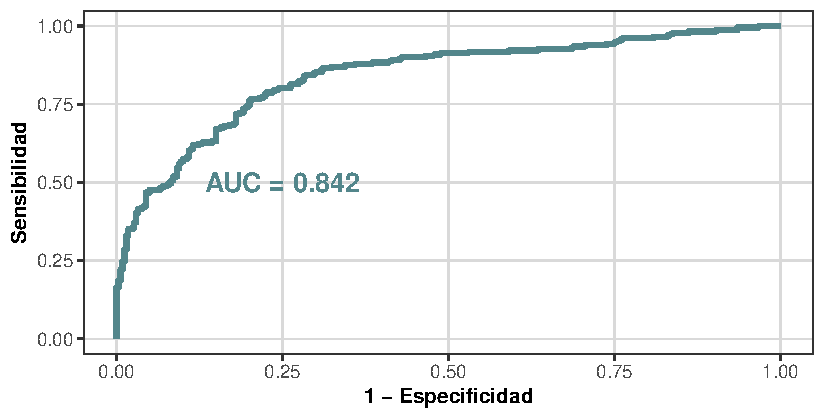
\includegraphics[keepaspectratio]{TpMLG_files/figure-pdf/unnamed-chunk-19-1.pdf}}

}

\caption{Gráfico probabilístico normal con residuos cuantil}

\end{figure}%

En dicho gráfico se observa que los puntos se alinean de manera adecuada
a lo largo de la línea de referencia, con leves dispersiones
concentradas en los extremos. Por lo tanto, no se evidencian desvíos
sistemáticos importantes respecto a la distribución teórica esperada, lo
que sugiere un ajuste globalmente satisfactorio del modelo.

\subsection{Estudio de la capacidad predictiva del
modelo}\label{estudio-de-la-capacidad-predictiva-del-modelo}

La capacidad predictiva del modelo se evaluó sobre el conjunto de
validación, es decir, sobre pasajeros que no participaron en la
estimación de los parámetros, de modo de obtener una medida de desempeño
que no esté sesgada por el ajuste. Con las probabilidades de
supervivencia estimadas para esas observaciones, se construyó la curva
ROC, que muestra cómo varían la sensibilidad (tasa de verdaderos
positivos) y la tasa de falsos positivos (1 - especificidad) al
modificar el punto de corte de clasificación. Esta curva permite
analizar el equilibrio entre ambos tipos de acierto y error, y es una
herramienta útil para elegir un umbral de clasificación adecuado.
Complementariamente, se calculó el área bajo la curva (AUC) como resumen
de la capacidad discriminante del modelo.

\begin{figure}[H]

{\centering \pandocbounded{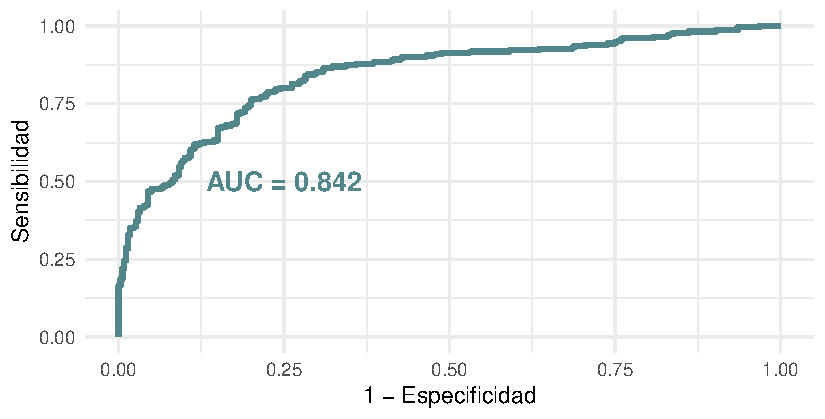
\includegraphics[keepaspectratio]{TpMLG_files/figure-pdf/unnamed-chunk-20-1.pdf}}

}

\caption{Curva ROC}

\end{figure}%

\begin{verbatim}
[1] 0.3798941
\end{verbatim}

El punto de corte seleccionado fue de 0.842, correspondiente al valor
que maximiza simultáneamente la sensibilidad y la especificidad del
modelo. Con este umbral se obtuvo la siguiente matriz de confusión, que
resume el desempeño del modelo en la clasificación de los casos:

{\def\LTcaptype{none} % do not increment counter
\begin{longtable}[]{@{}lcc@{}}
\toprule\noalign{}
\textbf{Predicho / Observado} & \textbf{No Sobrevivió} &
\textbf{Sobrevivió} \\
\midrule\noalign{}
\endhead
\bottomrule\noalign{}
\endlastfoot
\textbf{No Sobrevivió} & 69 & 13 \\
\textbf{Sobrevivió} & 15 & 44 \\
\end{longtable}
}

El modelo logró clasificar correctamente al 80\% de las observaciones
del conjunto de validación, con una sensibilidad del 77\% (proporción de
sobrevivientes correctamente identificados) y una especificidad del
82.1\% (proporción de no sobrevivientes correctamente clasificados).

\section{Resultados}\label{resultados}

En esta sección se presentan los principales hallazgos obtenidos a
partir del modelo final ajustado. En primer lugar, se exponen las
razones de odds estimadas para cada variable significativa, seguidas por
la representación gráfica de las mismas. Posteriormente, se incluyen las
curvas ajustadas que ilustran la probabilidad predicha de diabetes bajo
diferentes combinaciones de factores.

\#\# Razones de odds

Las razones de odds permiten cuantificar la variación en la probabilidad
de padecer diabetes ante cambios en las variables explicativas,
manteniendo constantes las demás condiciones.




\end{document}
